\documentclass{article}

\usepackage{graphicx}

\usepackage[tbtags]{amsmath}
\usepackage{amsthm}
\theoremstyle{plain}\newtheorem{thm}{Theorem}
\theoremstyle{definition}\newtheorem{defn}[thm]{Definition}

\title{Introduction to Splines}	
\author{Franz Webersberger}

\begin{document}

\maketitle

\newpage

\section*{B-splines}

\begin{defn}
Let $\tau_{1} \leq \cdots \leq \tau_{n}$ be an arbitrary sequence of nodes.
Then the B-splines $N_{i,k}(t)$ of order $k=1,\dots,n$ and $i=1,\dots,n-k$ 
are recursively defined by
\end{defn}

\begin{subequations}

	\begin{align}
			N_{i,1}(t) &:= 
					\begin{cases}
						1 & \text{if } \tau_{i} \leq t < \tau_{i+1}	\\
						0 & \text{else} \\
					\end{cases}
	\end{align}

	\begin{align}
			N_{i,k}(t) &:= 
				\frac{t-\tau_{i}}{\tau_{i+k-1}-\tau_{i}} N_{i,k-1}(t) + 
				\frac{\tau_{i+k}-t}{\tau_{i+k}-\tau_{i+1}} N_{i+1,k-1}(t)
	\end{align}							

\end{subequations}

\begin{figure}[h]

	\begin{center}
		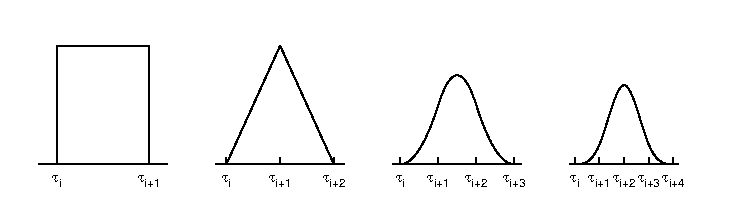
\includegraphics[width=12cm]{ni1234}
		\caption{B-splines of order $k=1,2,3,4$}
	\end{center}

	\begin{center}
		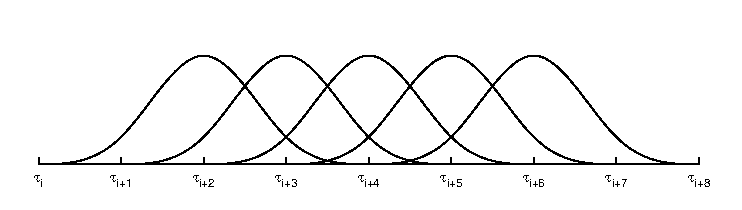
\includegraphics[width=12cm]{ni4-free}
		\caption{Uniform qubic $(k=4)$ B-splines}
	\end{center}

	\begin{center}
		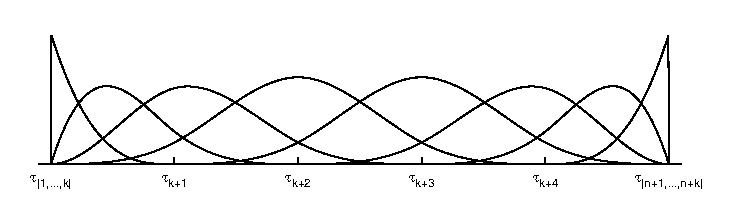
\includegraphics[width=12cm]{ni4-bound}
		\caption{Qubic B-splines with boundaries}
	\end{center}

\end{figure}
	

\end{document}

